% !TEX TS-program = pdflatexmk
\documentclass[12pt]{article}

% Layout.
\usepackage[top=1in, bottom=0.75in, left=1in, right=1in, headheight=1in, headsep=6pt]{geometry}

% Fonts.
\usepackage{mathptmx}
\usepackage[scaled=0.86]{helvet}
\renewcommand{\emph}[1]{\textsf{\textbf{#1}}}

% Misc packages.
\usepackage{amsmath,amssymb,latexsym}
\usepackage{graphicx,hyperref}
\usepackage{array}
\usepackage{xcolor}
\usepackage{multicol,tikz}
\usepackage{tabularx,colortbl,booktabs,xparse}
\usepackage{enumitem}

\renewcommand{\tabularxcolumn}[1]{m{#1}} % Centers X columns vertically

% Rotation: \rot[<angle>][<width>]{<stuff>}
\NewDocumentCommand{\rot}{O{45} O{1em} m}{\makebox[#2][l]{\rotatebox{#1}{#3}}}%

\usepackage{fancyhdr}
\pagestyle{fancy} 
\lhead{\large\sf\textbf{MATH F113X: Fair Division}}
\chead{\large\sf\textbf{lecture notes}}
\rhead{\large\sf\textbf{Lone Divider}}

\begin{document}
Goal: Review Divider-Chooser, motivate and introduce Lone-Divider
\begin{enumerate}
\item Recall from the previous worksheet: \quad Tom and Fred were given a cake worth \$12 that is equal parts strawberry, vanilla and chocolate. Their respective values summarized in the chart.\\
%%% VERSION2
\begin{tabular}{c@{\hspace{2em}}c@{\hspace{2em}}c}
% Table
\begin{tabular}[b]{c||ccc}
&vanilla&strawberry&chocolate\\
\hline \hline
Tom&\$ 6 & \$ 6 & \$ 0\\
Fred&\$ 2&\$ 4 & \$ 6\\
\end{tabular}
&
% Figure 1
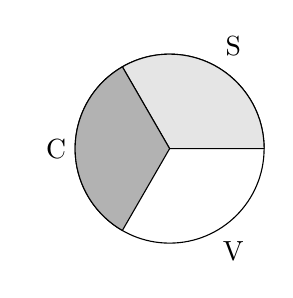
\begin{tikzpicture}[scale = .6, baseline={(0,0)}]
\def\r{2}
\draw (0,0) circle (\r cm);
\filldraw[fill= gray!20 ] (0,0) -- (0:\r) arc (0:120:\r) -- (0,0);
\path (60:2.5) node[]{{{ S}}};
\filldraw[fill = gray!60 ] (0,0) -- (120:\r) arc (120:240:\r) -- (0,0);
\path (120+60:2.5) node[]{{{ C}}};
\path (-60:2.5) node[]{{{ V}}};
\end{tikzpicture}
&
% Figure 2
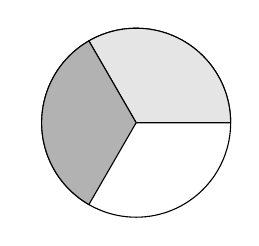
\begin{tikzpicture}[scale = .6, baseline={(0,0)}]
\def\r{2}
\draw (0,0) circle (\r cm);
\filldraw[fill= gray!20 ] (0,0) -- (0:\r) arc (0:120:\r) -- (0,0);
\filldraw[fill = gray!60 ] (0,0) -- (120:\r) arc (120:240:\r) -- (0,0);
\end{tikzpicture}
\end{tabular}

	\begin{enumerate}
	\item Divide the cake using Divider-Chooser assuming Tom is the divider. Determine the \emph{value} of the assigned share to each party. Use the pictures of the cake (above) to draw the outcome.)\\
%\begin{tikzpicture}[scale = .8]
%\def\r{2}
%\draw (0,0) circle (\r cm);
%\filldraw[fill= gray!20 ] (0,0) -- (0:\r) arc (0:120:\r) -- (0,0);
%\path (60:1) node[]{{{\scriptsize Strawberry}}};
%%\path node[right] (240:1) {{\scriptsize Strawberry}};
%\filldraw[fill = gray!60 ] (0,0) -- (120:\r) arc (120:240:\r) -- (0,0);
%\path (120+60:\r/2) node[]{{{\scriptsize Chocolate}}};
%\path (-60:\r/2) node[]{{{\scriptsize Vanilla}}};
%\end{tikzpicture}
\vfill	
	\item What happens if try to use Divider-Chooser with \emph{three} people? (Try Fred as divider.)\\
\\
%%% VERSION2
\begin{tabular}{c@{\hspace{2em}}c@{\hspace{2em}}cc}
% Table
\begin{tabular}[b]{c||ccc}
&V&S&C\\
\hline \hline
Tom&\$ 6 & \$ 6 & \$ 0\\
Fred&\$ 2&\$ 4 & \$ 6\\
Mary&\$8& \$ 0 & \$ 4\\
\end{tabular}
&
% Figure 1
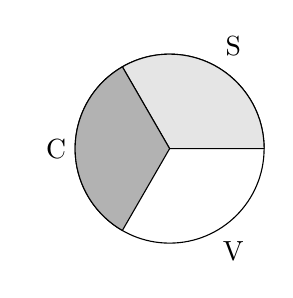
\begin{tikzpicture}[scale = .6, baseline={(0,0)}]
\def\r{2}
\draw (0,0) circle (\r cm);
\filldraw[fill= gray!20 ] (0,0) -- (0:\r) arc (0:120:\r) -- (0,0);
\path (60:2.5) node[]{{{ S}}};
\filldraw[fill = gray!60 ] (0,0) -- (120:\r) arc (120:240:\r) -- (0,0);
\path (120+60:2.5) node[]{{{ C}}};
\path (-60:2.5) node[]{{{ V}}};
\end{tikzpicture}
&
% Figure 2
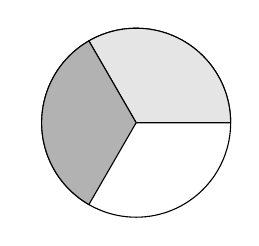
\begin{tikzpicture}[scale = .6, baseline={(0,0)}]
\def\r{2}
\draw (0,0) circle (\r cm);
\filldraw[fill= gray!20 ] (0,0) -- (0:\r) arc (0:120:\r) -- (0,0);
\filldraw[fill = gray!60 ] (0,0) -- (120:\r) arc (120:240:\r) -- (0,0);
\end{tikzpicture}
&
% Figure 3
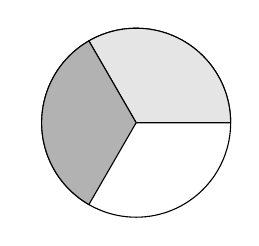
\begin{tikzpicture}[scale = .6, baseline={(0,0)}]
\def\r{2}
\draw (0,0) circle (\r cm);
\filldraw[fill= gray!20 ] (0,0) -- (0:\r) arc (0:120:\r) -- (0,0);
\filldraw[fill = gray!60 ] (0,0) -- (120:\r) arc (120:240:\r) -- (0,0);
\end{tikzpicture}
\end{tabular}

	\end{enumerate}
\vfill
\vfill

\item Why cake?
\vspace{0.5in}
\newpage
\item Lone-Divider Method (for $N$ people with $N \geq 3$).
\vspace*{-.1in}
	\begin{enumerate}[leftmargin=0.2in]
	\item[0.] \emph{Arbitrarily} pick a Divider.
	\item[1.] Divider divides the items into $N$ shares of equal value to them: $s_1,s_2, \cdots, s_N$.
	\item[2.] Remaining parties \textbf{declare} or \textbf{bid} on shares, $s_1,s_2, \cdots, s_N,$ they consider fair. 
	\item[3.] 
		\begin{enumerate}
		\item \textbf{IF} the $N$ shares can be divided such that each all get a fair share, then do so. 
		\item \textbf{IF NOT}, the Divider gets a \textbf{non-contested piece}. Remaining shares are recombined. Lone-Divider is restarted with $N-1$ parties.
		\item If only 2 parties remain, use Divider-Chooser.
		\end{enumerate}
	\end{enumerate}
\item \textbf{Example 1} Suppose Patrick, Chris, and Travis are splitting a pile of football memorabilia estimated to be worth \$300. It has been split into 3 shares and their respective values are summarized in the table.

(a) What is a fair share? \rule{2cm}{.5pt}
\begin{multicols}{2}
\begin{tabular}{c||c|c|c}
&$s_1$&$s_2$&$s_3$\\
\hline \hline
Patrick&\$50&\$150&\$100\\
Chris&\$70&\$70&\$160\\
Travis&\$100&\$100&\$100\\
\end{tabular} 

(b) Circle or highlight each individual's \textbf{bid} (the shares they would consider to be fair).\\

(c) Determine which person was the Divider.
\end{multicols}
(d) Determine the next steps of the Lone-Divider Method.
\vfill
\item \textbf{Example 2} Suppose Patrick, Chris, and Travis are splitting a pile of football memorabilia estimated to be worth \$300. It has been split into 3 (different) shares and their respective values are summarized in the table.
\begin{multicols}{2}
\begin{tabular}{c||c|c|c}
&$t_1$&$t_2$&$t_3$\\
\hline \hline
Patrick&\$100&\$100&\$100\\
Chris&\$90&\$40&\$170\\
Travis&\$50&\$90&\$160\\
\end{tabular} 

(a) Circle or highlight each individual's \textbf{bid} (the shares they would consider to be fair).\\

(b) Determine which person was the Divider.
\end{multicols}
(c) Determine the next steps of the Lone-Divider Method.
\vfill

\end{enumerate}
\end{document}